% Created 2019-09-25 Wed 22:12
% Intended LaTeX compiler: pdflatex
\documentclass[10pt,t]{beamer}
\usepackage[utf8]{inputenc}
\usepackage[T1]{fontenc}
\usepackage{graphicx}
\usepackage{grffile}
\usepackage{longtable}
\usepackage{wrapfig}
\usepackage{rotating}
\usepackage{amsmath}
\usepackage{textcomp}
\usepackage{amssymb}
\usepackage{capt-of}
\usepackage{hyperref}
\usetheme{default}
\author{L. Larrabee Strow}
\date{\today}
\title{\large Climate Hyperspectral InfraRed Product (CHIRP) Combining AIRS, CrIS, and IASI}
\subtitle{\footnotesize{AIRS Science Team Meeting}}
\date{\vspace{0.1in}\footnotesize{September 26, 2019 \vfill}}
\author{L. Larrabee Strow\inst{1,2}, Sergio DeSouza--Machado\inst{1,2}, Howard Motteler\inst{2}, Chris Hepplewhite\inst{2}, and Steven Buczkowski\inst{2}}
\institute[UMBC]{\inst{1} UMBC Physics Dept. \and \inst{2}UMBC JCET}
\input beamer_setup
\usetheme{metropolis}
\metroset{titleformat title=allcaps}
\renewcommand{\UrlFont}{\small\tt}
\renewcommand*{\UrlFont}{\footnotesize}
\tolerance=1000
\RequirePackage{fancyvrb}
\DefineVerbatimEnvironment{verbatim}{Verbatim}{fontsize=\footnotesize}
\hypersetup{
 pdfauthor={L. Larrabee Strow},
 pdftitle={\large Climate Hyperspectral InfraRed Product (CHIRP) Combining AIRS, CrIS, and IASI},
 pdfkeywords={},
 pdfsubject={},
 pdfcreator={Emacs 26.1 (Org mode 9.2)}, 
 pdflang={English}}
\begin{document}

\maketitle
\addtobeamertemplate{block begin}{
  \setlength{\parsep}{0pt}
  \setlength{\topsep}{3pt plus 2pt minus 2.5pt}
  \setlength{\itemsep}{0pt plus 0pt minus 2pt}
  \setlength{\partopsep}{2pt}
}

\begin{frame}[label={sec:org1e98192},shrink=20]{A Climate Hyperspectral InfraRed Product (CHIRP)}
\vspace{-0.1in}
\begin{block}{Motivation}
\begin{itemize}
\item Provide climate-level radiance time series spanning AIRS + CrIS, IASI
\item User friendly by using a single spectral instrument line shape (ILS)
\item A high-stability 25+ year long record of climate forcings and response
\item Level 2 retrievals can use a common Forward Model (RTA) and channel selection for consistency
\end{itemize}
\end{block}

\begin{block}{Three Products}
\begin{itemize}
\item CHIRP L1c: (radiances)
\begin{itemize}
\item Nearly ready
\item Q/A is the hard part
\end{itemize}
\item CHIRP L1c Gridded: (space/time gridded radiances)
\begin{itemize}
\item Simple product
\item May subdivide averaged/binned radiances into (a) nearly clear (b) mixed clear and cloudy, and (c) high (cold) deep optical depth clouds
\item This subdivision will greatly enhance surface, lower tropospheric retrievals
\end{itemize}
\item CHIRP Level 3: (geophysical anomalies)
\begin{itemize}
\item Retrieve geophysical anomalies
\item Start with radiance anomalies derived from CHIRP L1c Gridded
\end{itemize}
\end{itemize}
\end{block}
\end{frame}


\begin{frame}[label={sec:orga0cbe7d}]{Three Sensors Converted to Single Virtual Sensor}
\vspace{-0.2in}
\begin{columns}
\begin{column}{0.55\columnwidth}
\begin{block}{AIRS/CrIS/IASI Spectra}
\begin{center}
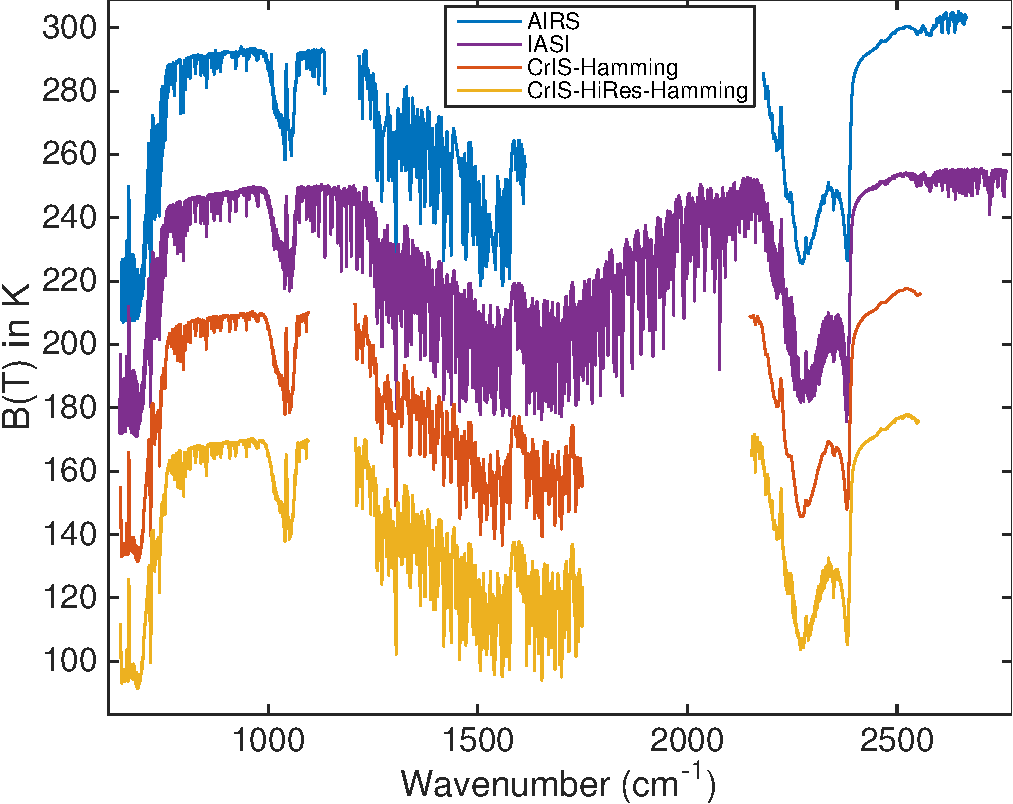
\includegraphics[width=\linewidth]{./Figs/Pdf/hyperall_hamming.pdf}
\end{center}
\end{block}
\end{column}


\begin{column}{0.55\columnwidth}
\begin{block}{CHIRP Spectrum (AIRS2CrIS)}
\begin{center}
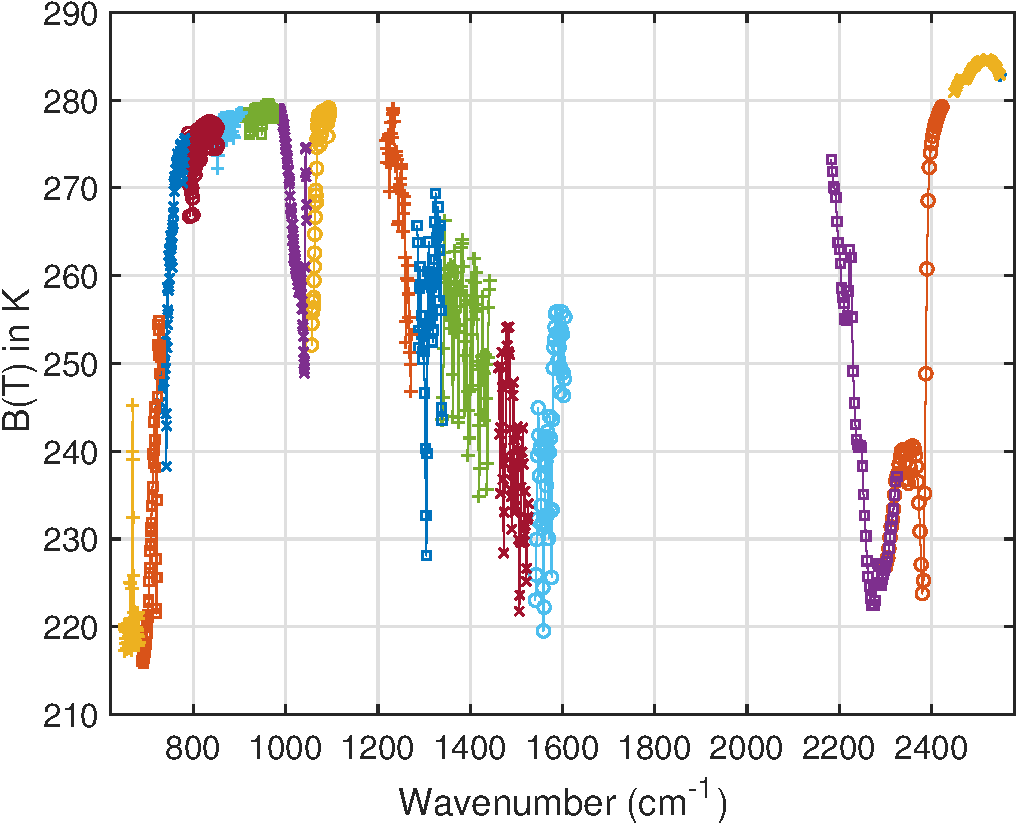
\includegraphics[width=\linewidth]{./Figs/Pdf/a2c_full.pdf}
\end{center}
\end{block}
\end{column}
\end{columns}

AIRS modules shown in different colors in CHIRP spectrum. This is CrIS-NSR, final CHIRP will be between CrIS NSR and FSR (MW/SW).
\end{frame}

\begin{frame}[label={sec:orgacd4c0d}]{CHIRP L1c}
\begin{itemize}
\item Uses AIRS L1c and CrIS L1b (and IASI) as inputs
\item Granule in, granule out
\item Common insrument line shape (ILS), \textbf{allows us to correct for inter-instrument radiance offsets}
\item CHIRP noise often lower than input noise, normalize to a common level?
\item Signifiant Q/A effort: AIRS Q/A influences CrIS Q/A flags
\end{itemize}
\end{frame}

\begin{frame}[label={sec:org195f52e}]{CHIRP L1c Gridded}
\begin{itemize}
\item Likely most important long-term climate data record
\item Simple gridding of CHIRP L1c
\item 16 day bins (orbit repeat cycle)
\item Nominal 1x1 degree grid?
\item Gridded radiance noise included
\item Radiometric offset correction for AIRS to match CrIS mean secant angle (0.2-0.3K correction)
\end{itemize}
\end{frame}

\begin{frame}[label={sec:org3614f62}]{CHIRP Level 3 (Gridded) Geophysical Anomalies}
\begin{itemize}
\item Input is CHIRP L1c Gridded
\item Create anomalies in radiance space before geophysical retrievals to enhance error  traceability
\item Approach minimizes sensitivity to a-priori estimates (i.e. use zero for T, \water, \ozone a-priori estimates)
\item Minimze sampling biases due to clouds
\item Designed for quick reprocessing, essential for climate products
\end{itemize}
\end{frame}

\begin{frame}[label={sec:org17583f1}]{CHIRP Processing Flow}
\vspace{-0.2in}
\begin{center}
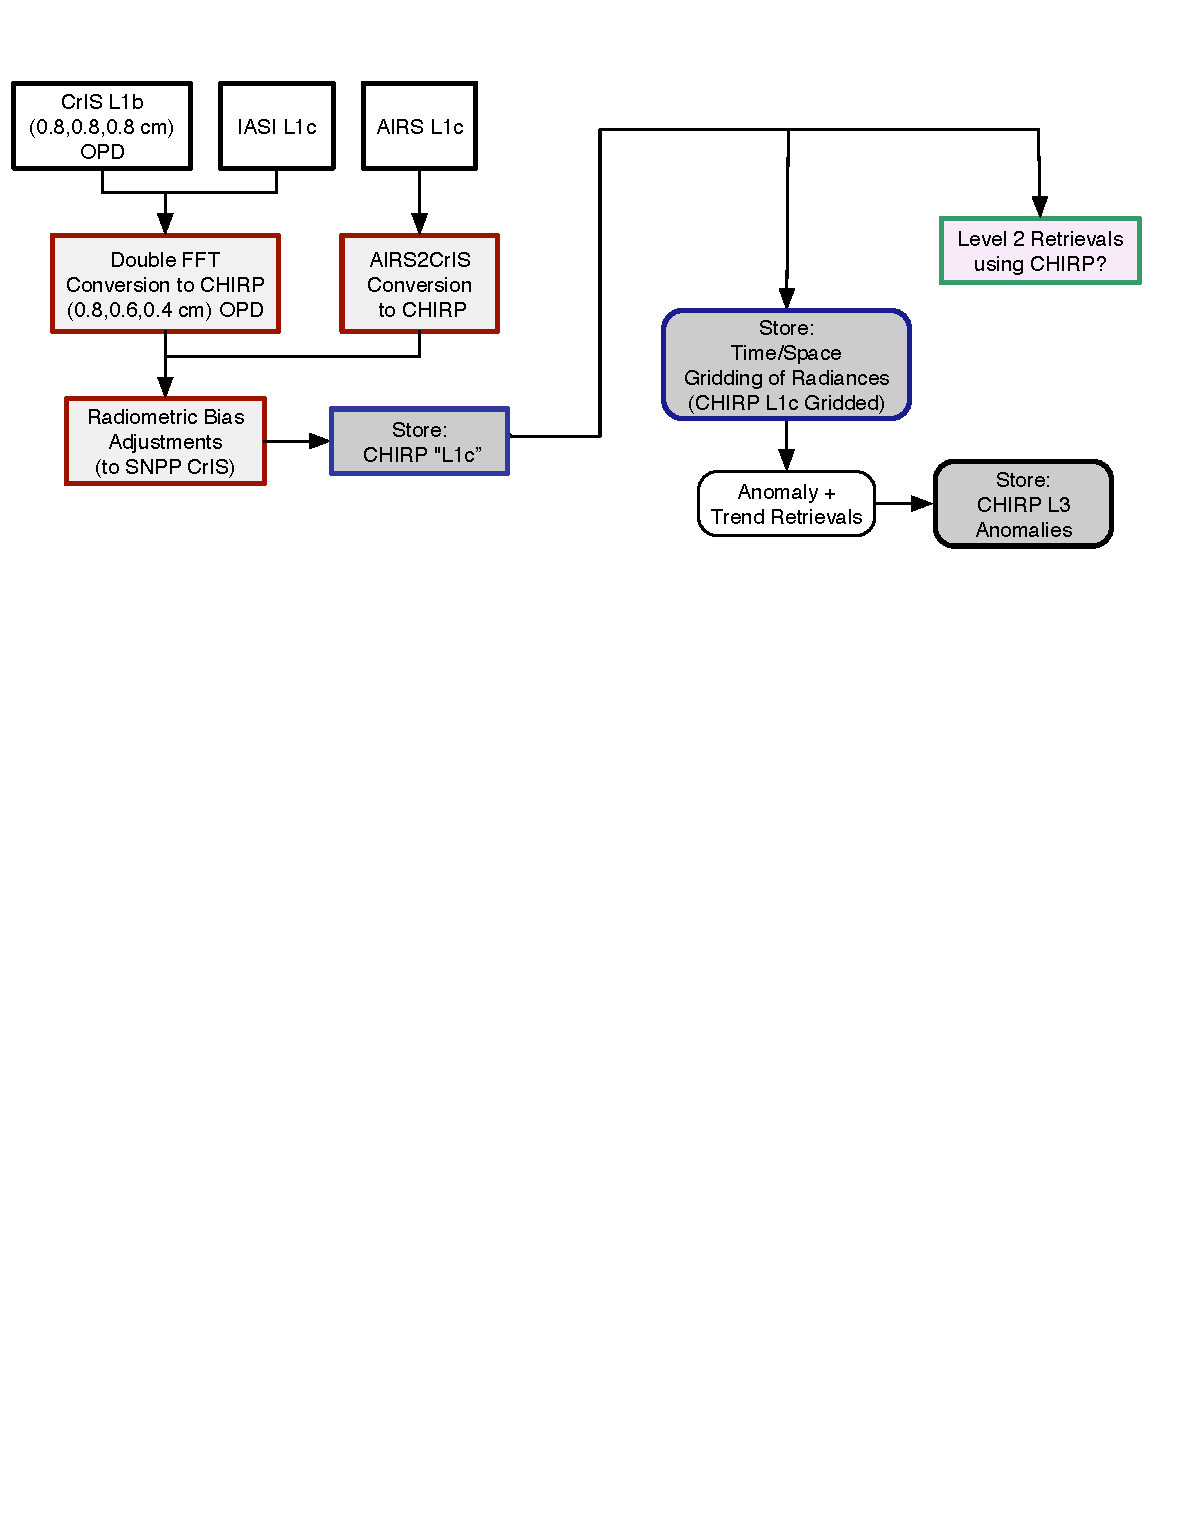
\includegraphics[width=1.0\linewidth]{./airs2cris_stm_talk1_landscape.pdf}
\end{center}

CHIRP: (Common or Climate) Hyperspectral InfraRed Product

\vspace{0.05in}

\small
\begin{itemize}
\item CrIS High-Res OPD = 0.8/0.8/0.8 cm
\item CHIRP "OPD" = 0.8/0.6/0.4 cm  \hspace{0.1in} (Allows AIRS conversion to CrIS)
\item CHIRP MW/SW 75\%/50\% lower resolution than CrIS
\end{itemize}
\end{frame}


\begin{frame}[label={sec:org78aa51e}]{AIRS2CrIS Algorithm}
\vspace{-0.15in}
\begin{small}
\begin{itemize}
\item Simple deconvolution to 0.1 \wn grid
\item \(S_a r = r_A\), \(r_o = S_a^{-1} r_A\) using Moore-Penrose pseudoinverse
\item \(r_{A2C} = S_c \circledast r_o\)
\item Small additional terms using linear regression (mostly bias)
\item Errors below assume AIRS ILS functions are perfect
\end{itemize}
\end{small}
\vspace{-0.25in}
\begin{columns}
\begin{column}{0.55\columnwidth}
\begin{block}{\footnotesize AIRS2CrIS Mean Error (std. similar)}
\vspace{-0.1in}
\begin{center}
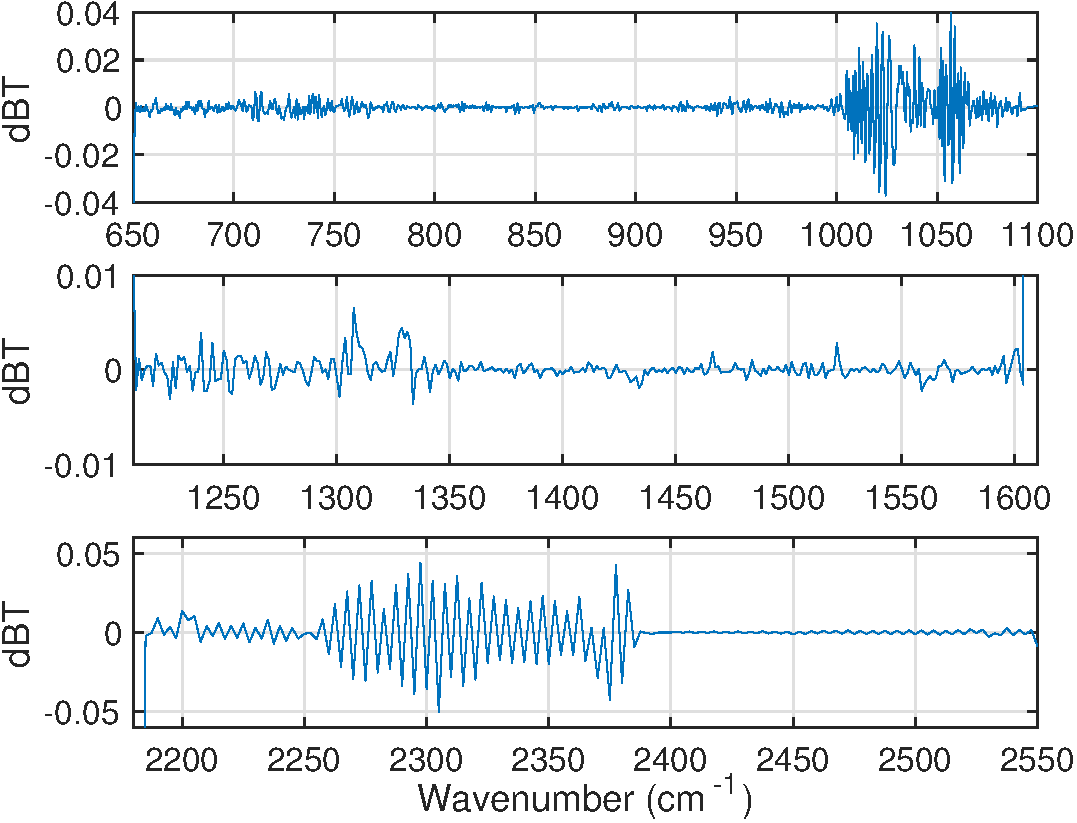
\includegraphics[width=0.95\linewidth]{./Figs/Pdf/ap_decon_corr.pdf}
\end{center}
\end{block}
\end{column}

\begin{column}{0.55\columnwidth}
\begin{block}{\footnotesize AIRS2CrIS Noise}
\vspace{-0.1in}
\begin{center}
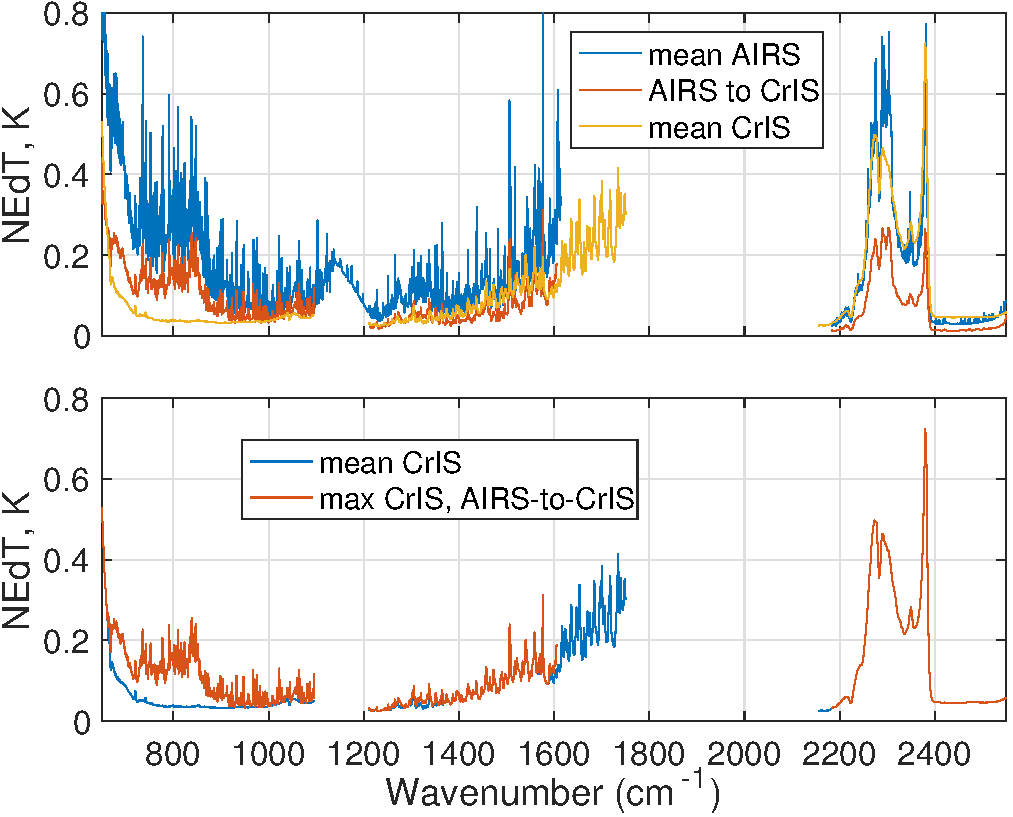
\includegraphics[width=0.95\linewidth]{./Figs/Pdf/a2cris_nedt.pdf}
\end{center}
\end{block}
\end{column}
\end{columns}

\vspace{-0.1in}
\small Shortwave sounding region max noise dominated by CrIS
\end{frame}

\begin{frame}[label={sec:orge611577}]{Radiometric Corrections Applied to AIRS}
\vspace{-0.1in}
\begin{itemize}
\item CrIS-like ILS is CHIRP standard
\item We convert AIRS to CrIS ILS, and apply inter-instrument radiometric offsets to create a seamless record
\end{itemize}
\begin{center}
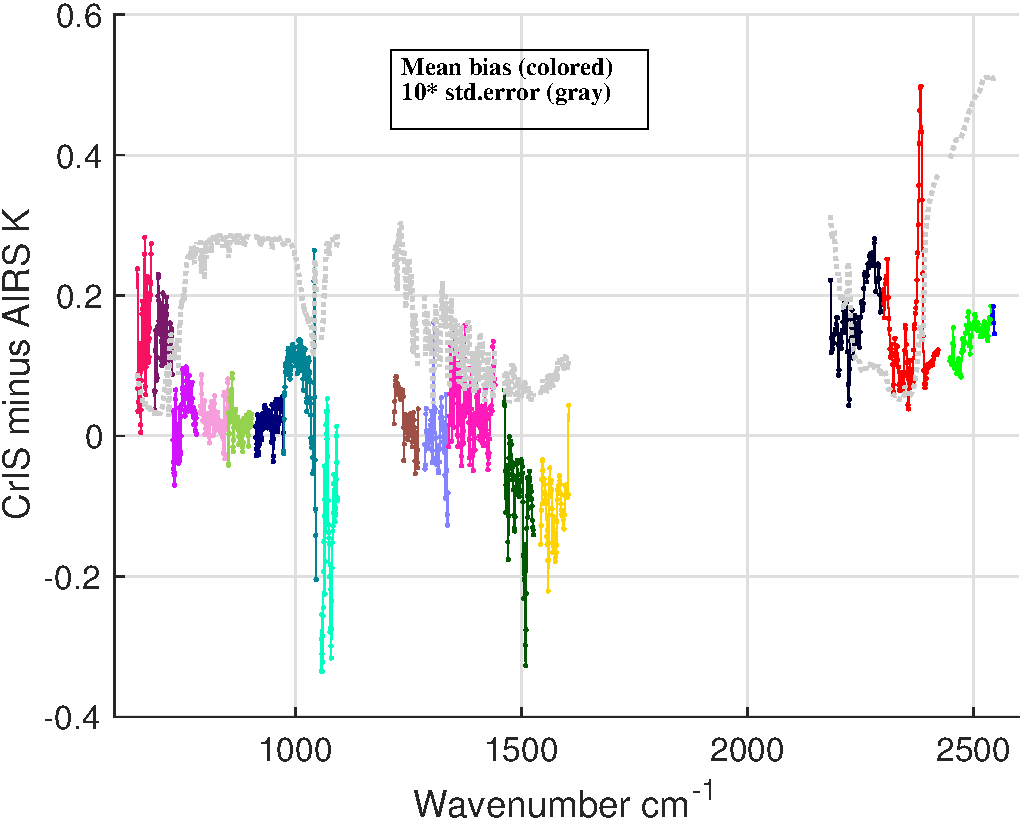
\includegraphics[width=0.7\linewidth]{./ac_sno_2018_bias_stderr_coloraslp.pdf}
\end{center}
\end{frame}

\begin{frame}[label={sec:org9e92127}]{Anomaly and Trend Approach:}
First: generate radiance anomalies \(dBT(t)\).\\
Then perform geophysical anomaly retrievals.\\

\vspace{0.1in}

Linear solution for trends with a-priori state = 0 given by,
\begin{displaymath}
dx(t) =  \left(K^T S_{\epsilon}^{-1} K + R^{-1}\right)^{-1} \left(K^T S_{\epsilon}^{-1} dBT(t)\right)
\end{displaymath}

\begin{itemize}
\item \emph{dx(t)} are the atmospheric state vector anomalies
\item \emph{K} are the B(T) Jacobians
\item \(S_{\epsilon}\) is the observation error covariance matrix (noise)
\item \emph{R} combines empirical regularization (Tikonov L1-type) and the \emph{a-priori} covariance-based terms
\end{itemize}

Sergio showed zonally averaged dx(t) samples yesterday\\

\small
\vspace{0.1in}
\begin{itemize}
\item Cloud parameter Jacobians may be derived from MERRA-2 (or ERA5)
\item Or, if necessary retrievals of \(x(t)\), at least for cloud top heights and amounts
\end{itemize}
\end{frame}

\begin{frame}[label={sec:org3f823d4}]{Level 2 Retrievals using CHIRP}
\begin{itemize}
\item CHIRP L1c could be input for the AIRS/CrIS Level 2 product
\item Removes instrument bias differences
\item Removes retrieval differences due to different RTAs
\item Level 2 validation may be more straightfoward using this approach
\end{itemize}
\end{frame}

\begin{frame}[label={sec:org3a0c2c9}]{Conclusions}
\begin{itemize}
\item We hope to have CHIRP L1c algorithm ready in several months
\begin{itemize}
\item File formats almost done
\item Q/A issues and noise normalization still being worked out
\end{itemize}
\item CHIRP L1c Gridded will soon follow, relatively easy to develop
\item CHIRP Level 3 geophysical anomalies will require further development
\begin{itemize}
\item Hope to have CHIRP Level 3 mature in 1 year
\end{itemize}
\end{itemize}
\end{frame}
\end{document}